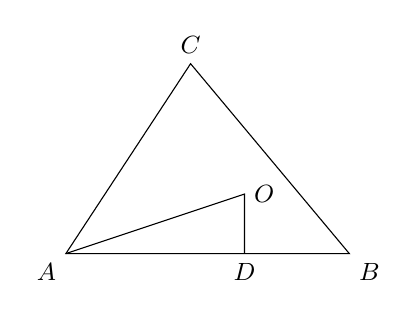
\begin{tikzpicture}[scale=.72, every node/.style={font=\small}]
  \coordinate (A) at (0,0); \coordinate (B) at (5,0);
  \coordinate (C) at (2.20,3.35); \coordinate (D) at (3.15,0); \coordinate (O) at (3.15,1.05);
  \draw (A)--(B)--(C)--cycle;
  \draw (A)--(O)--(D);
  \foreach \p/\pos in {A/below left,B/below right,C/above,D/below,O/right}
    \node[\pos] at (\p) {$\p$};
\end{tikzpicture}
